\documentclass[hyperref={pdfpagelabels=false}]{beamer}

\usepackage{ragged2e}
\renewcommand{\raggedright}{\leftskip=0pt \rightskip=0pt plus 0cm}

\usepackage{lmodern}
\usepackage{fontspec}
\usepackage{xeCJK}
\setCJKmainfont{Noto Sans CJK TC}
\setCJKsansfont{Noto Sans CJK TC}
\setCJKmonofont{Noto Sans Mono CJK TC}

\usepackage[english]{babel}
\usepackage{amsmath,amssymb,amsfonts,amsthm}

\hypersetup{
  colorlinks=true,
  urlcolor=blue,
  citecolor=blue,
  pdfborder={0 0 0}
}

\usepackage{accsupp}
\newcommand{\emptyaccsupp}[1]{\BeginAccSupp{ActualText={}}#1\EndAccSupp{}}

\usepackage{tikz}
\usetikzlibrary{arrows,positioning,shapes}
\usepackage{booktabs}
\usepackage{xcolor}
\usepackage{graphicx}

% ---- lstlisting: R language ----------------------------------------
\usepackage{listings}

\lstdefinelanguage{R}{
  morekeywords=[1]{if,else,for,while,function,return,library,require,
                   TRUE,FALSE,NULL,NA,Inf,NaN},
  morekeywords=[2]{install.packages,p_load,rm,list,ls,cat,print,
                   head,tail,summary,
                   rast,crop,mask,vect,ext,res,crs,values,ncell,
                   extract,global,
                   gadm,st_as_sf,st_transform,st_drop_geometry,
                   st_crs,st_geometry,
                   ggplot,aes,geom_spatraster,geom_sf,
                   scale_fill_viridis_c,scale_fill_gradient2,
                   coord_sf,labs,theme_void,theme,ggsave,
                   element_text,unit,plot_annotation,plot_layout,
                   mutate,select,filter,arrange,desc,group_by,
                   summarise,rename,rename_with,left_join,
                   pivot_wider,row_number,setNames,all_of,
                   write_csv,write_dta,
                   file.path,dir.create,paste,paste0,log,median,
                   quantile,abs,range,c,names,tail},
  morestring=[b]",
  morestring=[b]',
  morecomment=[l]{\#},
  sensitive=true,
}

\lstdefinestyle{rstyle}{
  language=R,
  basicstyle=\scriptsize\ttfamily,
  keywordstyle={\color{NavyBlue}},
  keywordstyle=[2]{\color{NavyBlue}},
  stringstyle=\color{Maroon},
  commentstyle=\color{OliveGreen},
  numbers=none,
  breaklines=true,
  frame=single,
  backgroundcolor=\color{gray!5},
  showstringspaces=false,
}

\lstset{style=rstyle}
% -------------------------------------------------------------------

\beamertemplatefootpagenumber

\usetheme{Boadilla}
\usecolortheme{seahorse}
\setbeamertemplate{footline}{%
  \hfill\usebeamercolor[fg]{page number in head/foot}%
  \usebeamerfont{page number in head/foot}%
  \insertframenumber\,/\,\inserttotalframenumber\hspace{1em}\vspace{2pt}%
}

\beamersetuncovermixins{\opaqueness<1>{25}}{\opaqueness<2->{15}}

%=====================================================================
\title[]{Satellite Data: Practical Implementation}
\author{Prof. Tzu-Ting Yang \\ 楊子霆}
\institute{Institute of Economics, Academia Sinica \\ 中央研究院經濟研究所}
\date{\today}
%=====================================================================

\begin{document}

\begin{frame}{}
  \titlepage
\end{frame}


%=====================================================================
\title[]{Overview}
\author{}
\institute{}
\date{}
\begin{frame}{}
  \titlepage
\end{frame}


\begin{frame}{What We Do Today}
\begin{itemize}
  \item \textbf{Goal:} read satellite raster data, process it in R,
        and aggregate to a township-level panel ready for regression
  \vspace{0.3cm}
  \item \textbf{Data: Harmonized Nighttime Lights}
  \vspace{0.15cm}
  \begin{itemize}
    \item Harmonized DMSP-OLS / VIIRS simulated NTL (GeoTIFF)
    \vspace{0.1cm}
    \item Compare Taiwan in 2013 vs.\ 2024
    \vspace{0.1cm}
    \item Aggregate to township level (鄉鎮市區, $\approx$368 units)
  \end{itemize}
  \vspace{0.3cm}
  \item \textbf{Key concepts covered:}
  \vspace{0.15cm}
  \begin{itemize}
    \item Raster data structure and GeoTIFF format
    \vspace{0.1cm}
    \item Coordinate reference systems (CRS)
    \vspace{0.1cm}
    \item Crop, mask, and extract operations
  \end{itemize}
  \vspace{0.3cm}
  \item \textbf{Output files}
  \vspace{0.15cm}
  \begin{itemize}
    \item Maps (PNG) $\Rightarrow$ \texttt{S3\_Geo\_data/figure/}
    \vspace{0.05cm}
    \item Township data $\Rightarrow$ \texttt{taiwan\_ntl\_township\_wide.csv / .dta}
  \end{itemize}
\end{itemize}
\end{frame}


\begin{frame}{R Script}
\begin{itemize}
  \item Full code: \texttt{Class\_Data/R\_code/nighttime\_lights\_taiwan\_v3.R}
  \vspace{0.3cm}
  \item Key packages:
  \vspace{0.1cm}
  \begin{center}
  \small
  \begin{tabular}{ll}
    \toprule
    \textbf{Package}    & \textbf{Role} \\
    \midrule
    \texttt{terra}      & Raster operations (read, crop, mask, extract) \\
    \texttt{tidyterra}  & \texttt{ggplot2} + \texttt{terra} integration \\
    \texttt{sf}         & Vector spatial data (shapefiles) \\
    \texttt{geodata}    & Download GADM administrative boundaries \\
    \texttt{ggplot2}    & Map visualisation \\
    \texttt{patchwork}  & Combine multiple ggplots \\
    \texttt{haven}      & Export to Stata \texttt{.dta} \\
    \bottomrule
  \end{tabular}
  \end{center}
\end{itemize}
\end{frame}


%=====================================================================
\title[]{Nighttime Lights Data}
\author{}
\institute{}
\date{}
\begin{frame}{}
  \titlepage
\end{frame}


\begin{frame}{Nighttime Lights as an Economic Indicator}
\begin{itemize}
  \item \textbf{Why nighttime lights?}
  \vspace{0.2cm}
  \begin{itemize}
    \item Light intensity at night is a strong proxy for economic activity
    \vspace{0.1cm}
    \item Publicly available, globally consistent, fine spatial resolution
  \end{itemize}
  \vspace{0.3cm}
  \item \textbf{Key reference:}
  \vspace{0.1cm}
  \begin{itemize}
    \item Henderson, Storeygard, and Weil (2012),
          ``\textbf{Measuring Economic Growth from Outer Space}'', AER
    \vspace{0.1cm}
    \item Nighttime lights predict GDP growth at both national and
          sub-national levels
  \end{itemize}
  \vspace{0.3cm}
  \item \textbf{Advantages over official statistics:}
  \vspace{0.1cm}
  \begin{itemize}
    \item Available for regions where official GDP data are poor or absent
    \vspace{0.1cm}
    \item Can capture \emph{within-country} spatial variation at fine scale
    \vspace{0.1cm}
    \item Consistent over time and across countries
  \end{itemize}
\end{itemize}
\end{frame}


\begin{frame}{Two Generations of Nighttime Lights Data}
\begin{center}
\small
\begin{tabular}{lcc}
  \toprule
  & \textbf{DMSP-OLS} & \textbf{NASA Black Marble (VIIRS)} \\
  \midrule
  Sensor        & DMSP / OLS      & Suomi-NPP VIIRS DNB \\
  Coverage      & 1992–2013       & 2012–present \\
  Resolution    & $\sim$1 km      & 500 m \\
  Radiometric   & 6-bit (0–63)    & 14-bit, calibrated nW/sr/cm$^2$ \\
  Saturation    & Yes (urban)     & No \\
  Moonlight corr.& No             & Yes \\
  Cloud mask    & Partial         & Yes \\
  \bottomrule
\end{tabular}
\end{center}
\vspace{0.2cm}
\begin{itemize}
  \item \textbf{Problem:} DMSP ends in 2013; VIIRS starts in 2012
        --- the two series are \emph{not} directly comparable
  \vspace{0.15cm}
  \item \textbf{Solution:} use a \textbf{harmonized} dataset that
        intercalibrates both sensors onto a common scale
\end{itemize}
\end{frame}


\begin{frame}{Harmonized DMSP-OLS / VIIRS Dataset}
\begin{itemize}
  \item \textbf{Data we use:} Harmonized simulated VIIRS (``simVIIRS'')
  \vspace{0.2cm}
  \begin{itemize}
    \item Based on Li et al.\ (2020), \textit{Remote Sensing of Environment}
    \vspace{0.1cm}
    \item DMSP-OLS data intercalibrated and converted to VIIRS-like scale
    \vspace{0.1cm}
    \item Coverage: 1992–2024, global, $\sim$1 km resolution
  \end{itemize}
  \vspace{0.3cm}
  \item \textbf{File naming:}
  \vspace{0.1cm}
  \begin{itemize}
    \item \texttt{Harmonized\_DN\_NTL\_\{year\}\_simVIIRS.tif}
    \vspace{0.1cm}
    \item ``DN'' = Digital Number (unitless brightness index)
    \vspace{0.1cm}
    \item One GeoTIFF per year, global extent
  \end{itemize}
  \vspace{0.3cm}
  \item \textbf{Format: GeoTIFF}
  \vspace{0.1cm}
  \begin{itemize}
    \item Standard raster format readable by \texttt{terra}, QGIS, Python, etc.
    \vspace{0.1cm}
    \item Contains embedded georeferencing information (CRS + extent)
  \end{itemize}
\end{itemize}
\end{frame}


\begin{frame}{What is a Raster?}
\begin{itemize}
  \item A \textbf{raster} is a grid of regularly spaced cells (pixels),
        each storing one or more numeric values
  \vspace{0.3cm}
  \item Each cell covers a fixed geographic area (the \textbf{resolution}),
        e.g.\ $\sim$1 km $\times$ 1 km
  \vspace{0.3cm}
  \item A raster is fully described by:
  \vspace{0.15cm}
  \begin{center}
  \small
  \begin{tabular}{ll}
    \toprule
    \textbf{Property} & \textbf{Example (our data)} \\
    \midrule
    Extent   & Global: $-180^\circ$ to $180^\circ$, $-90^\circ$ to $90^\circ$ \\
    Resolution & $\approx 0.0083^\circ$ ($\approx 926$ m at equator) \\
    CRS      & WGS84 (EPSG:4326) \\
    Dimensions & $\sim$43200 cols $\times$ 21600 rows \\
    Values   & Digital Number (DN), 0–63 \\
    \bottomrule
  \end{tabular}
  \end{center}
  \vspace{0.3cm}
  \item In R, the \texttt{terra} package represents rasters as
        \texttt{SpatRaster} objects
\end{itemize}
\end{frame}


%=====================================================================
\title[]{Coordinate Reference Systems}
\author{}
\institute{}
\date{}
\begin{frame}{}
  \titlepage
\end{frame}


\begin{frame}{Why CRS Matters}
\begin{itemize}
  \item Every spatial dataset --- raster or vector --- is referenced
        to a \textbf{coordinate reference system (CRS)}
  \vspace{0.3cm}
  \item The CRS defines how coordinates $(x, y)$ map to locations
        on the Earth's surface
  \vspace{0.3cm}
  \item \textbf{Common mistake:} overlaying two layers with
        \emph{different} CRS
  \vspace{0.15cm}
  \begin{itemize}
    \item Polygons will not align with the raster grid
    \vspace{0.1cm}
    \item Extraction results will be wrong or empty
  \end{itemize}
  \vspace{0.3cm}
  \item \textbf{Rule:} always check and harmonize CRS before any
        spatial operation
  \vspace{0.15cm}
  \begin{itemize}
    \item Check: \texttt{terra::crs(r)} / \texttt{sf::st\_crs(shp)}
    \vspace{0.1cm}
    \item Transform vector: \texttt{sf::st\_transform(shp, crs = 4326)}
    \vspace{0.1cm}
    \item Reproject raster: \texttt{terra::project(r, "EPSG:4326")}
  \end{itemize}
\end{itemize}
\end{frame}


\begin{frame}{Two Types of Coordinate Systems}
\begin{itemize}
  \item \textbf{Geographic Coordinate System (GCS)}
  \vspace{0.15cm}
  \begin{itemize}
    \item Measures location in \textbf{degrees}: longitude / latitude
    \vspace{0.1cm}
    \item Three-dimensional angular system referenced to a datum
    \vspace{0.1cm}
    \item Example: WGS84 --- longitude $\in [-180^\circ, 180^\circ]$,
          latitude $\in [-90^\circ, 90^\circ]$
    \vspace{0.1cm}
    \item \textbf{Taipei:} $24.57^\circ$ N, $121.32^\circ$ E
  \end{itemize}
  \vspace{0.35cm}
  \item \textbf{Projected Coordinate System (PCS)}
  \vspace{0.15cm}
  \begin{itemize}
    \item Flattens the globe onto a 2D plane; units in \textbf{meters}
    \vspace{0.1cm}
    \item Needed for accurate distance and area calculations
    \vspace{0.1cm}
    \item Example: TWD97 (Taiwan Datum 1997, EPSG:3826) ---
          used by government shapefiles
    \vspace{0.1cm}
    \item All projections introduce some distortion --- choose one
          appropriate for your region
  \end{itemize}
\end{itemize}
\end{frame}


\begin{frame}{EPSG Codes}
\begin{itemize}
  \item \textbf{EPSG} (European Petroleum Survey Group) maintains a
        registry of standardized CRS codes
  \vspace{0.3cm}
  \begin{center}
  \small
  \begin{tabular}{lll}
    \toprule
    \textbf{EPSG} & \textbf{Name} & \textbf{Usage} \\
    \midrule
    4326 & WGS84         & Global; GPS, most satellite data \\
    3826 & TWD97 / TM2   & Taiwan government data \\
    3857 & Web Mercator  & Web maps (Google Maps, OSM) \\
    32651 & UTM Zone 51N & East Asia, metric distances \\
    \bottomrule
  \end{tabular}
  \end{center}
  \vspace{0.3cm}
  \item \textbf{In this practical:}
  \vspace{0.15cm}
  \begin{itemize}
    \item NTL GeoTIFF $\Rightarrow$ WGS84 (EPSG:4326)
    \vspace{0.1cm}
    \item GADM shapefile downloaded via \texttt{geodata::gadm()}
          $\Rightarrow$ WGS84 (EPSG:4326)
    \vspace{0.1cm}
    \item Both layers already match $\Rightarrow$ no reprojection needed
  \end{itemize}
\end{itemize}
\end{frame}


\begin{frame}[fragile]{CRS in R: Checking and Transforming}
\begin{lstlisting}
# Check raster CRS
terra::crs(tif_2013, describe = TRUE)
# -> name: "WGS 84", authority: "EPSG", code: "4326"

# Check vector CRS
sf::st_crs(tw_sf)$epsg   # -> 4326

# Transform vector to WGS84 (if needed)
tw_sf <- sf::st_transform(tw_sf, crs = 4326)

# Reproject raster (if CRS mismatch)
# r_wgs84 <- terra::project(r, "EPSG:4326")
\end{lstlisting}
\begin{itemize}
  \item The \texttt{terra} $\leftrightarrow$ \texttt{sf} interface:
        use \texttt{terra::vect()} to convert \texttt{sf}
        $\to$ \texttt{SpatVector} for raster operations
\end{itemize}
\end{frame}


%=====================================================================
\title[]{Taiwan Administrative Boundaries}
\author{}
\institute{}
\date{}
\begin{frame}{}
  \titlepage
\end{frame}


\begin{frame}{GADM: Administrative Boundaries}
\begin{itemize}
  \item \textbf{GADM} (Global Administrative Areas) provides
        free, consistent administrative boundary files for all countries
  \vspace{0.15cm}
  \begin{itemize}
    \item Website: \href{https://gadm.org}{\texttt{gadm.org}}
    \vspace{0.1cm}
    \item Downloaded in R with \texttt{geodata::gadm()} (with local caching)
  \end{itemize}
  \vspace{0.3cm}
  \item \textbf{GADM levels for Taiwan:}
  \vspace{0.15cm}
  \begin{center}
  \small
  \begin{tabular}{cll}
    \toprule
    \textbf{Level} & \textbf{Unit} & \textbf{Count} \\
    \midrule
    0 & Country (Taiwan)           & 1 \\
    1 & Province / Special Municipality & 7 \\
    2 & County / City (縣市)        & 22 \\
    3 & Township / District (鄉鎮市區) & $\approx$368 \\
    \bottomrule
  \end{tabular}
  \end{center}
  \vspace{0.3cm}
  \item We use \textbf{Level 3} to get township-level statistics
  \vspace{0.1cm}
  \begin{itemize}
    \item Key column: \texttt{NAME\_1} (county),
          \texttt{NAME\_3} (township name)
  \end{itemize}
\end{itemize}
\end{frame}


\begin{frame}[fragile]{Downloading Taiwan Shapefile in R}
\begin{lstlisting}
# geodata::gadm() downloads GADM and caches locally
# Second run reads from cache (no internet needed)
tw_sf <- geodata::gadm("TWN",
                        level = 3,
                        path  = gadm_cache) |>
  sf::st_as_sf() |>
  sf::st_transform(crs = 4326)

cat("Townships:", nrow(tw_sf))   # 368

# Name columns available
names(tw_sf)[grepl("^NAME_", names(tw_sf))]
# "NAME_1" "NAME_2" "NAME_3"
# NAME_1 = county, NAME_3 = township
\end{lstlisting}
\begin{itemize}
  \item \texttt{st\_transform(crs = 4326)} ensures WGS84 ---
        same CRS as the NTL raster
\end{itemize}
\end{frame}


%=====================================================================
\title[]{R Code Walkthrough}
\author{}
\institute{}
\date{}
\begin{frame}{}
  \titlepage
\end{frame}


\begin{frame}[fragile]{Step 0: Load Packages}
\begin{lstlisting}
if (!require("pacman")) install.packages("pacman")
library(pacman)

p_load(
  terra,      # Raster core: rast, crop, mask, extract
  tidyterra,  # geom_spatraster (ggplot2 + terra)
  sf,         # Vector data: shapefiles, CRS transform
  geodata,    # gadm() for administrative boundaries
  tidyverse,  # ggplot2, dplyr, etc.
  haven,      # Export .dta (Stata)
  patchwork,  # Combine ggplots side by side
  scales      # squish (color scale capping)
)
\end{lstlisting}
\end{frame}


\begin{frame}[fragile]{Step 1: Read GeoTIFF with \texttt{terra::rast()}}
\begin{lstlisting}
# terra::rast() reads metadata only (lazy loading)
# Pixels are loaded on demand -> memory efficient
tif_2013 <- terra::rast(
  file.path(ntl_dir,
            "Harmonized_DN_NTL_2013_simVIIRS.tif"))
tif_2024 <- terra::rast(
  file.path(ntl_dir,
            "Harmonized_DN_NTL_2024_simVIIRS.tif"))

# Inspect the raster
print(tif_2013)
cat("CRS:", terra::crs(tif_2013, describe=TRUE)$name)
cat("Extent:", as.vector(terra::ext(tif_2013)))
cat("Resolution:", terra::res(tif_2013))
\end{lstlisting}
\begin{itemize}
  \item \texttt{terra::rast()} returns a \texttt{SpatRaster} object
  \vspace{0.1cm}
  \item Always inspect CRS and extent before any spatial operations
\end{itemize}
\end{frame}


\begin{frame}[fragile]{Step 2: Load Shapefile (GADM Level 3)}
\begin{lstlisting}
tw_sf <- geodata::gadm("TWN", level = 3,
                        path = gadm_cache) |>
  sf::st_as_sf() |>
  sf::st_transform(crs = 4326)  # harmonize CRS

# Convert sf -> SpatVector for terra operations
tw_vect <- terra::vect(tw_sf)
\end{lstlisting}
\vspace{0.1cm}
\begin{itemize}
  \item \texttt{terra} operates on \texttt{SpatVector}; \texttt{sf} uses
        \texttt{sf} objects --- \texttt{terra::vect()} bridges the two
  \vspace{0.2cm}
  \item Both NTL raster and shapefile are now in WGS84 $\Rightarrow$
        CRS is consistent
\end{itemize}
\end{frame}


\begin{frame}[fragile]{Step 3: Crop and Mask to Taiwan}
\begin{lstlisting}
# Two-step spatial subsetting
#  crop()  : rectangular clip to bounding box (fast)
#  mask()  : zero out pixels outside polygons

ntl_2013 <- tif_2013 |>
  terra::crop(tw_vect) |>
  terra::mask(tw_vect)

ntl_2024 <- tif_2024 |>
  terra::crop(tw_vect) |>
  terra::mask(tw_vect)

names(ntl_2013) <- "ntl_2013"
names(ntl_2024) <- "ntl_2024"
\end{lstlisting}
\begin{itemize}
  \item Why two steps? \texttt{crop()} first reduces the global raster
        to Taiwan's bounding box; \texttt{mask()} then sets pixels
        outside Taiwan's polygon to \texttt{NA}
  \item Doing \texttt{mask()} alone on the full global raster would be
        very slow
\end{itemize}
\end{frame}


\begin{frame}[fragile]{Step 4: Visualize --- Raster Maps}
\begin{lstlisting}
# Log transform: NTL is right-skewed
ntl_2013_log <- log(ntl_2013 + 1)
names(ntl_2013_log) <- "log_ntl"

# Map function using geom_spatraster (tidyterra)
make_ntl_map <- function(r_log, title_text, tw_sf,
                          midpoint) {
  ggplot() +
    geom_spatraster(data = r_log) +
    geom_sf(data = tw_sf, fill = NA,
            color = "gray60", linewidth = 0.1) +
    scale_fill_gradient2(
      low="black", mid="orange", high="white",
      midpoint = midpoint, na.value="transparent",
      name = "log(NTL+1)") +
    coord_sf(expand = FALSE) +
    labs(title = title_text, x = NULL, y = NULL) +
    theme_void(base_size = 11)
}
\end{lstlisting}
\end{frame}


\begin{frame}[fragile]{Step 4 (cont.): Save Maps}
\begin{lstlisting}
# Shared midpoint for comparable color scales
all_log_vals <- c(
  terra::values(ntl_2013_log, na.rm = TRUE),
  terra::values(ntl_2024_log, na.rm = TRUE))
mid_shared <- median(all_log_vals[all_log_vals > 0],
                     na.rm = TRUE)

p_2013 <- make_ntl_map(ntl_2013_log,
  "Taiwan NTL 2013", tw_sf, mid_shared)
p_2024 <- make_ntl_map(ntl_2024_log,
  "Taiwan NTL 2024", tw_sf, mid_shared)

# Side-by-side comparison
p_compare <- p_2013 + p_2024 +
  plot_layout(guides = "collect")

ggsave(file.path(fig_path, "ntl_taiwan_compare.png"),
       p_compare, width = 11, height = 6, dpi = 300)
\end{lstlisting}
\end{frame}


\begin{frame}[fragile]{Step 4 (cont.): Change Map}
\begin{lstlisting}
ntl_change        <- ntl_2024 - ntl_2013
names(ntl_change) <- "change"
ntl_change        <- terra::mask(ntl_change, tw_vect)

# Cap at 99th percentile to handle outliers
change_cap <- quantile(
  abs(terra::values(ntl_change, na.rm = TRUE)),
  0.99, na.rm = TRUE)

p_change <- ggplot() +
  geom_spatraster(data = ntl_change) +
  geom_sf(data = tw_sf, fill = NA,
          color = "gray50", linewidth = 0.1) +
  scale_fill_gradient2(
    low = "royalblue3", mid = "white",
    high = "firebrick3", midpoint = 0,
    limits = c(-change_cap, change_cap),
    oob = scales::squish,
    na.value = "transparent", name = "Change (DN)")
\end{lstlisting}
\begin{itemize}
  \item Blue = decreased; Red = increased brightness
\end{itemize}
\end{frame}


\begin{frame}[fragile]{Step 5: Extract Township-Level Statistics}
\begin{lstlisting}
# terra::extract(): assign each raster pixel to a polygon
# fun = NULL -> returns all pixel values per polygon
extract_stats <- function(r, tw_vect) {
  ex <- terra::extract(r, tw_vect,
                        fun = NULL, na.rm = TRUE)
  layer_nm <- names(r)
  ex |>
    rename(value = all_of(layer_nm)) |>
    group_by(ID) |>
    summarise(
      ntl_mean   = mean(value,   na.rm = TRUE),
      ntl_sum    = sum(value,    na.rm = TRUE),
      ntl_sd     = sd(value,     na.rm = TRUE),
      ntl_median = median(value, na.rm = TRUE),
      n_pixels   = n(),
      n_valid    = sum(!is.na(value)),
      .groups = "drop")
}
\end{lstlisting}
\end{frame}


\begin{frame}[fragile]{Step 5 (cont.): Join and Compute Changes}
\begin{lstlisting}
stats_2013 <- extract_stats(ntl_2013, tw_vect) |>
  rename_with(~ paste0(., "_2013"), -ID)
stats_2024 <- extract_stats(ntl_2024, tw_vect) |>
  rename_with(~ paste0(., "_2024"), -ID)

# Township metadata (county + township name)
tw_meta <- tw_sf |>
  sf::st_drop_geometry() |>
  mutate(ID = row_number()) |>
  select(ID, county = NAME_1, township = NAME_3)

# Wide-format dataset: one row per township
tw_ntl <- tw_meta |>
  left_join(stats_2013, by = "ID") |>
  left_join(stats_2024, by = "ID") |>
  mutate(
    ntl_change_mean = ntl_mean_2024 - ntl_mean_2013,
    ntl_pct_change  = (ntl_mean_2024 - ntl_mean_2013) /
                      (ntl_mean_2013 + 1) * 100)
\end{lstlisting}
\end{frame}


\begin{frame}[fragile]{Step 6: Export Data}
\begin{lstlisting}
# Each year as a separate long-format file
tw_ntl_2013 <- tw_ntl |>
  select(county, township,
         ntl_mean = ntl_mean_2013,
         ntl_sum  = ntl_sum_2013,
         ntl_sd   = ntl_sd_2013) |>
  mutate(year = 2013)

write_csv(tw_ntl_2013,
  file.path(out_path, "taiwan_ntl_township_2013.csv"))
haven::write_dta(tw_ntl_2013,
  file.path(out_path, "taiwan_ntl_township_2013.dta"))

# Wide-format: both years, one row per township
write_csv(tw_ntl,
  file.path(out_path, "taiwan_ntl_township_wide.csv"))
haven::write_dta(tw_ntl,
  file.path(out_path, "taiwan_ntl_township_wide.dta"))
\end{lstlisting}
\begin{itemize}
  \item \texttt{.dta} can be opened in Stata with \texttt{use}
\end{itemize}
\end{frame}


%=====================================================================
\title[]{Results}
\author{}
\institute{}
\date{}
\begin{frame}{}
  \titlepage
\end{frame}


\begin{frame}{Taiwan Nighttime Lights: 2013}
  \begin{center}
    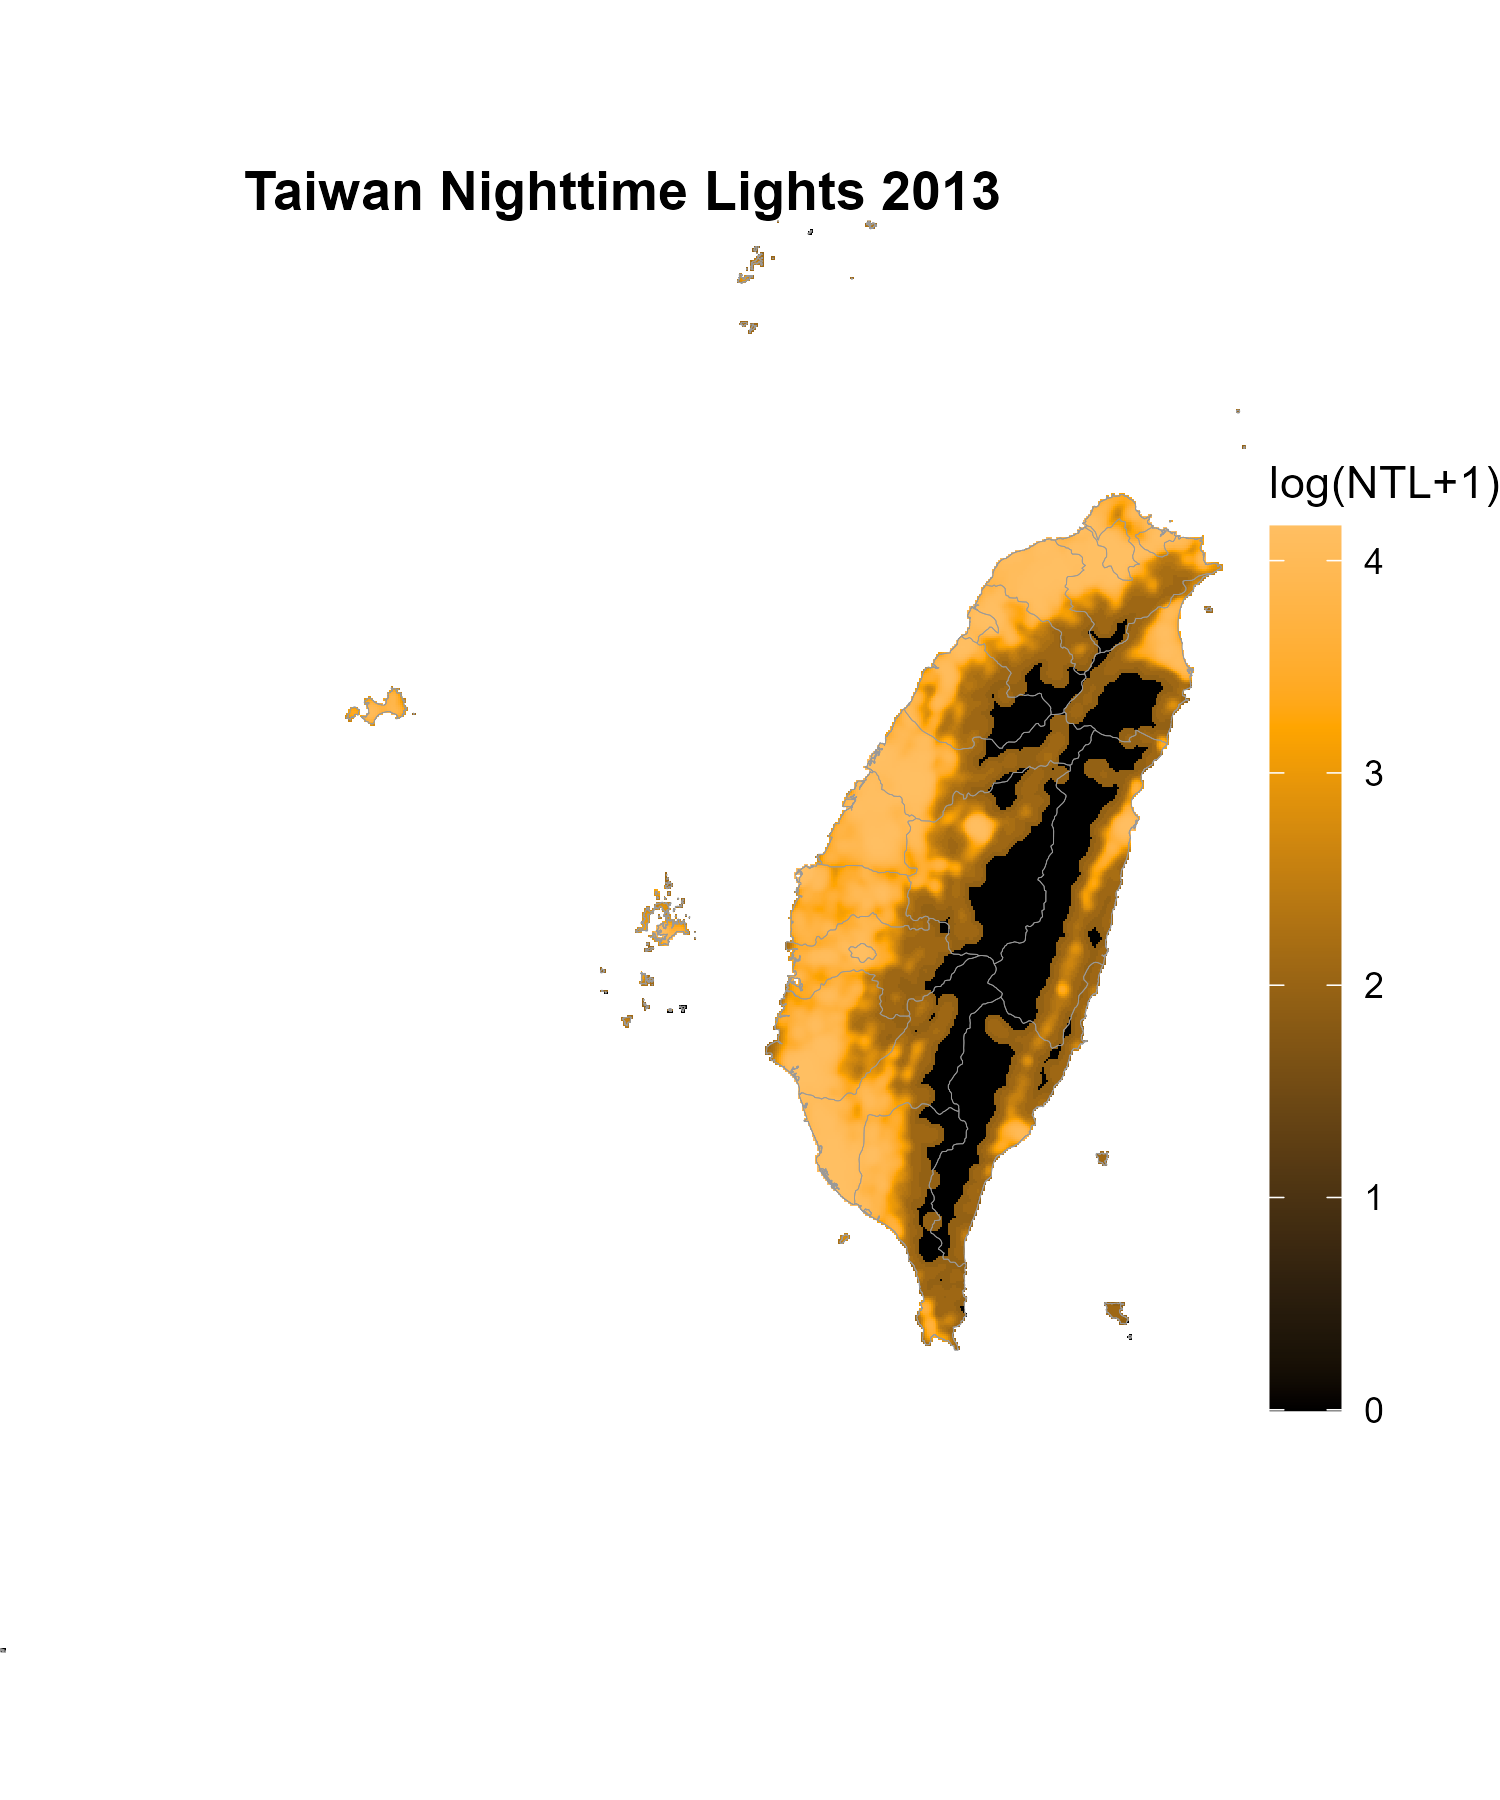
\includegraphics[width=0.75\textwidth]{figure/ntl_taiwan_2013.png}
  \end{center}
\end{frame}


\begin{frame}{Taiwan Nighttime Lights: 2024}
  \begin{center}
    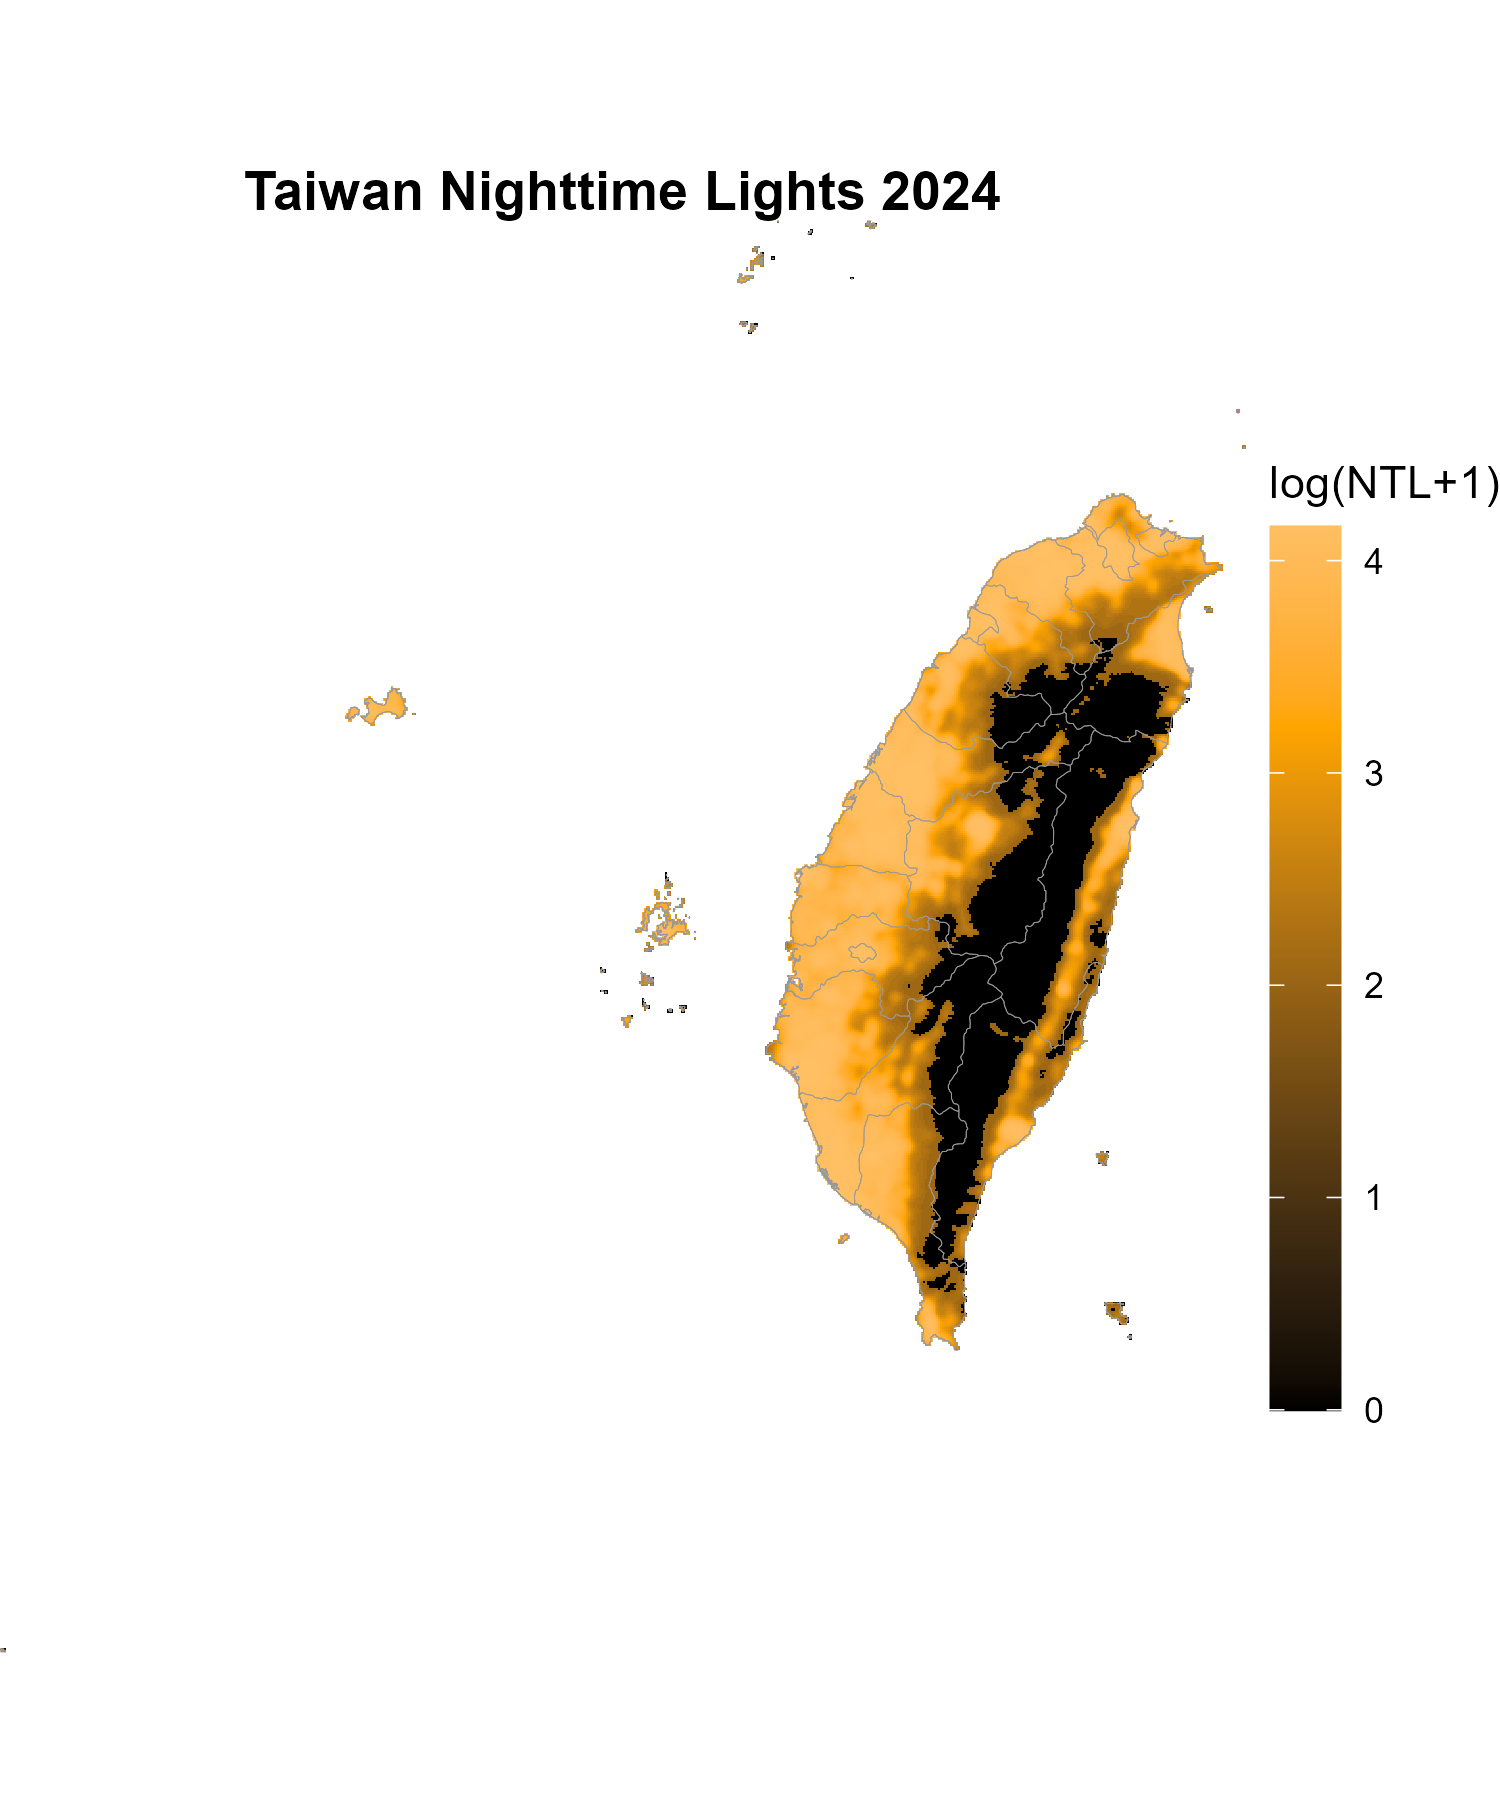
\includegraphics[width=0.75\textwidth]{figure/ntl_taiwan_2024.png}
  \end{center}
\end{frame}


\begin{frame}{Taiwan Nighttime Lights: 2013 vs.\ 2024}
  \begin{center}
    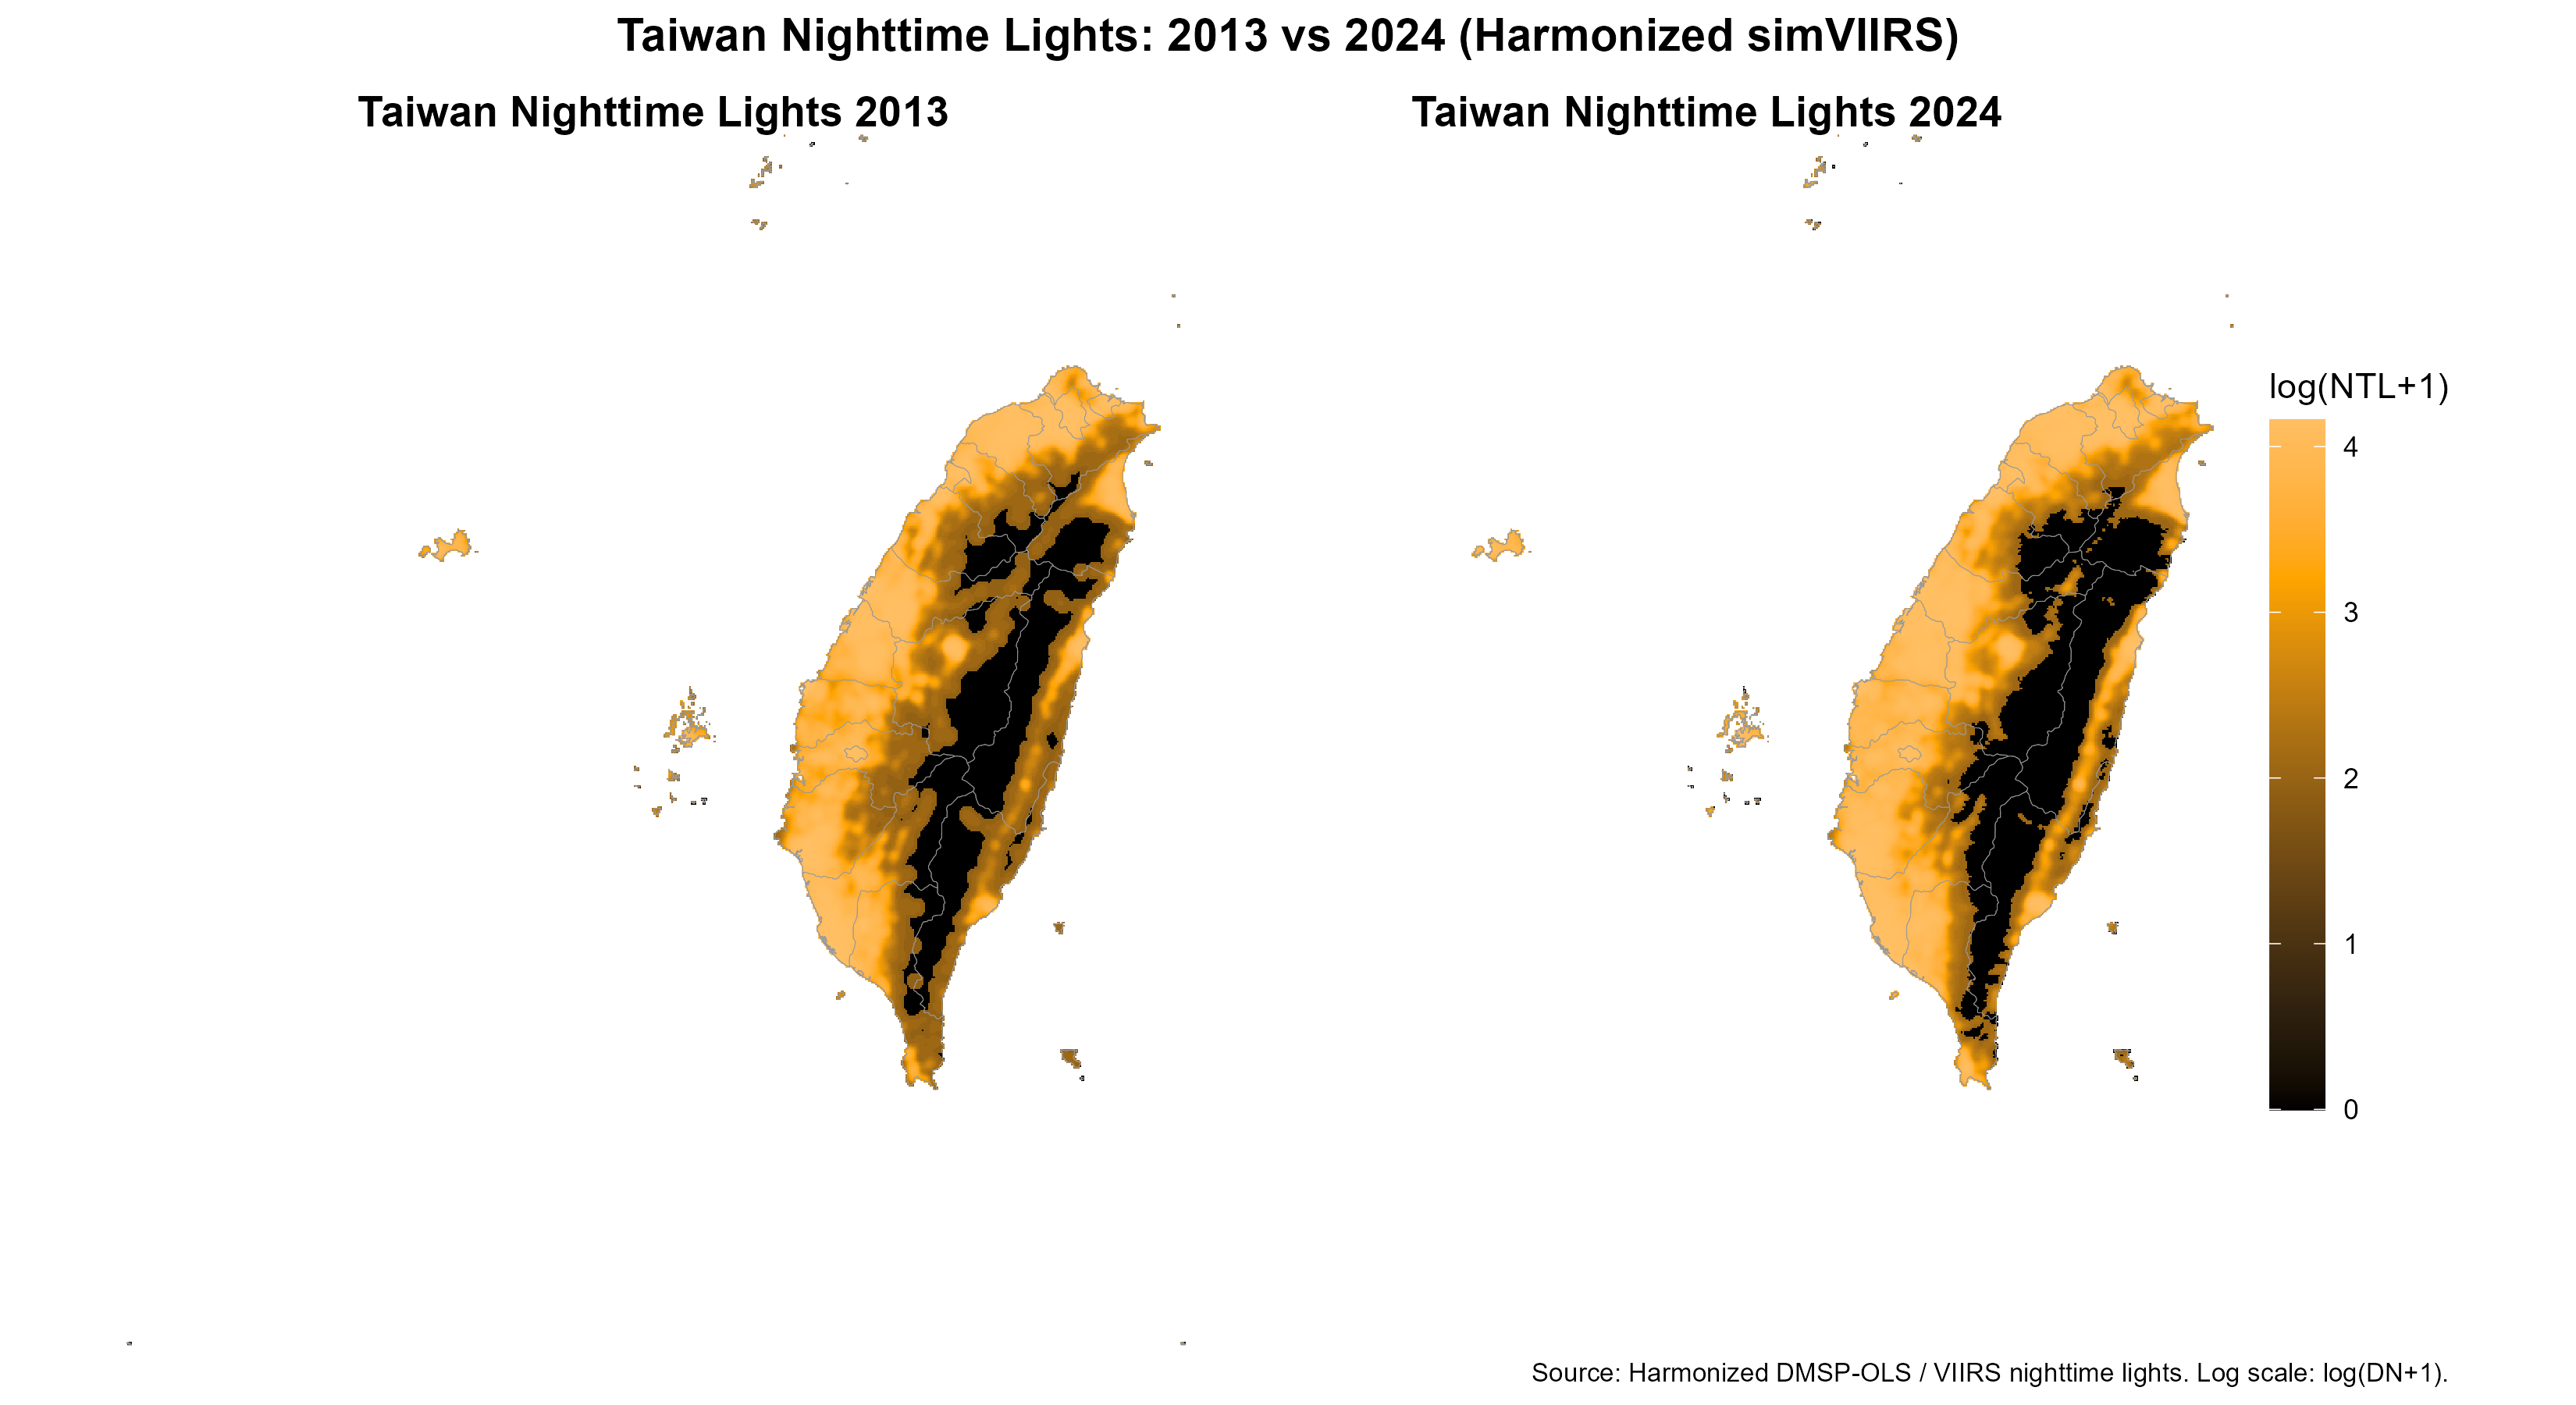
\includegraphics[width=\textwidth]{figure/ntl_taiwan_compare.png}
  \end{center}
\end{frame}


\begin{frame}{Change in Nighttime Lights: 2024 $-$ 2013}
  \begin{center}
    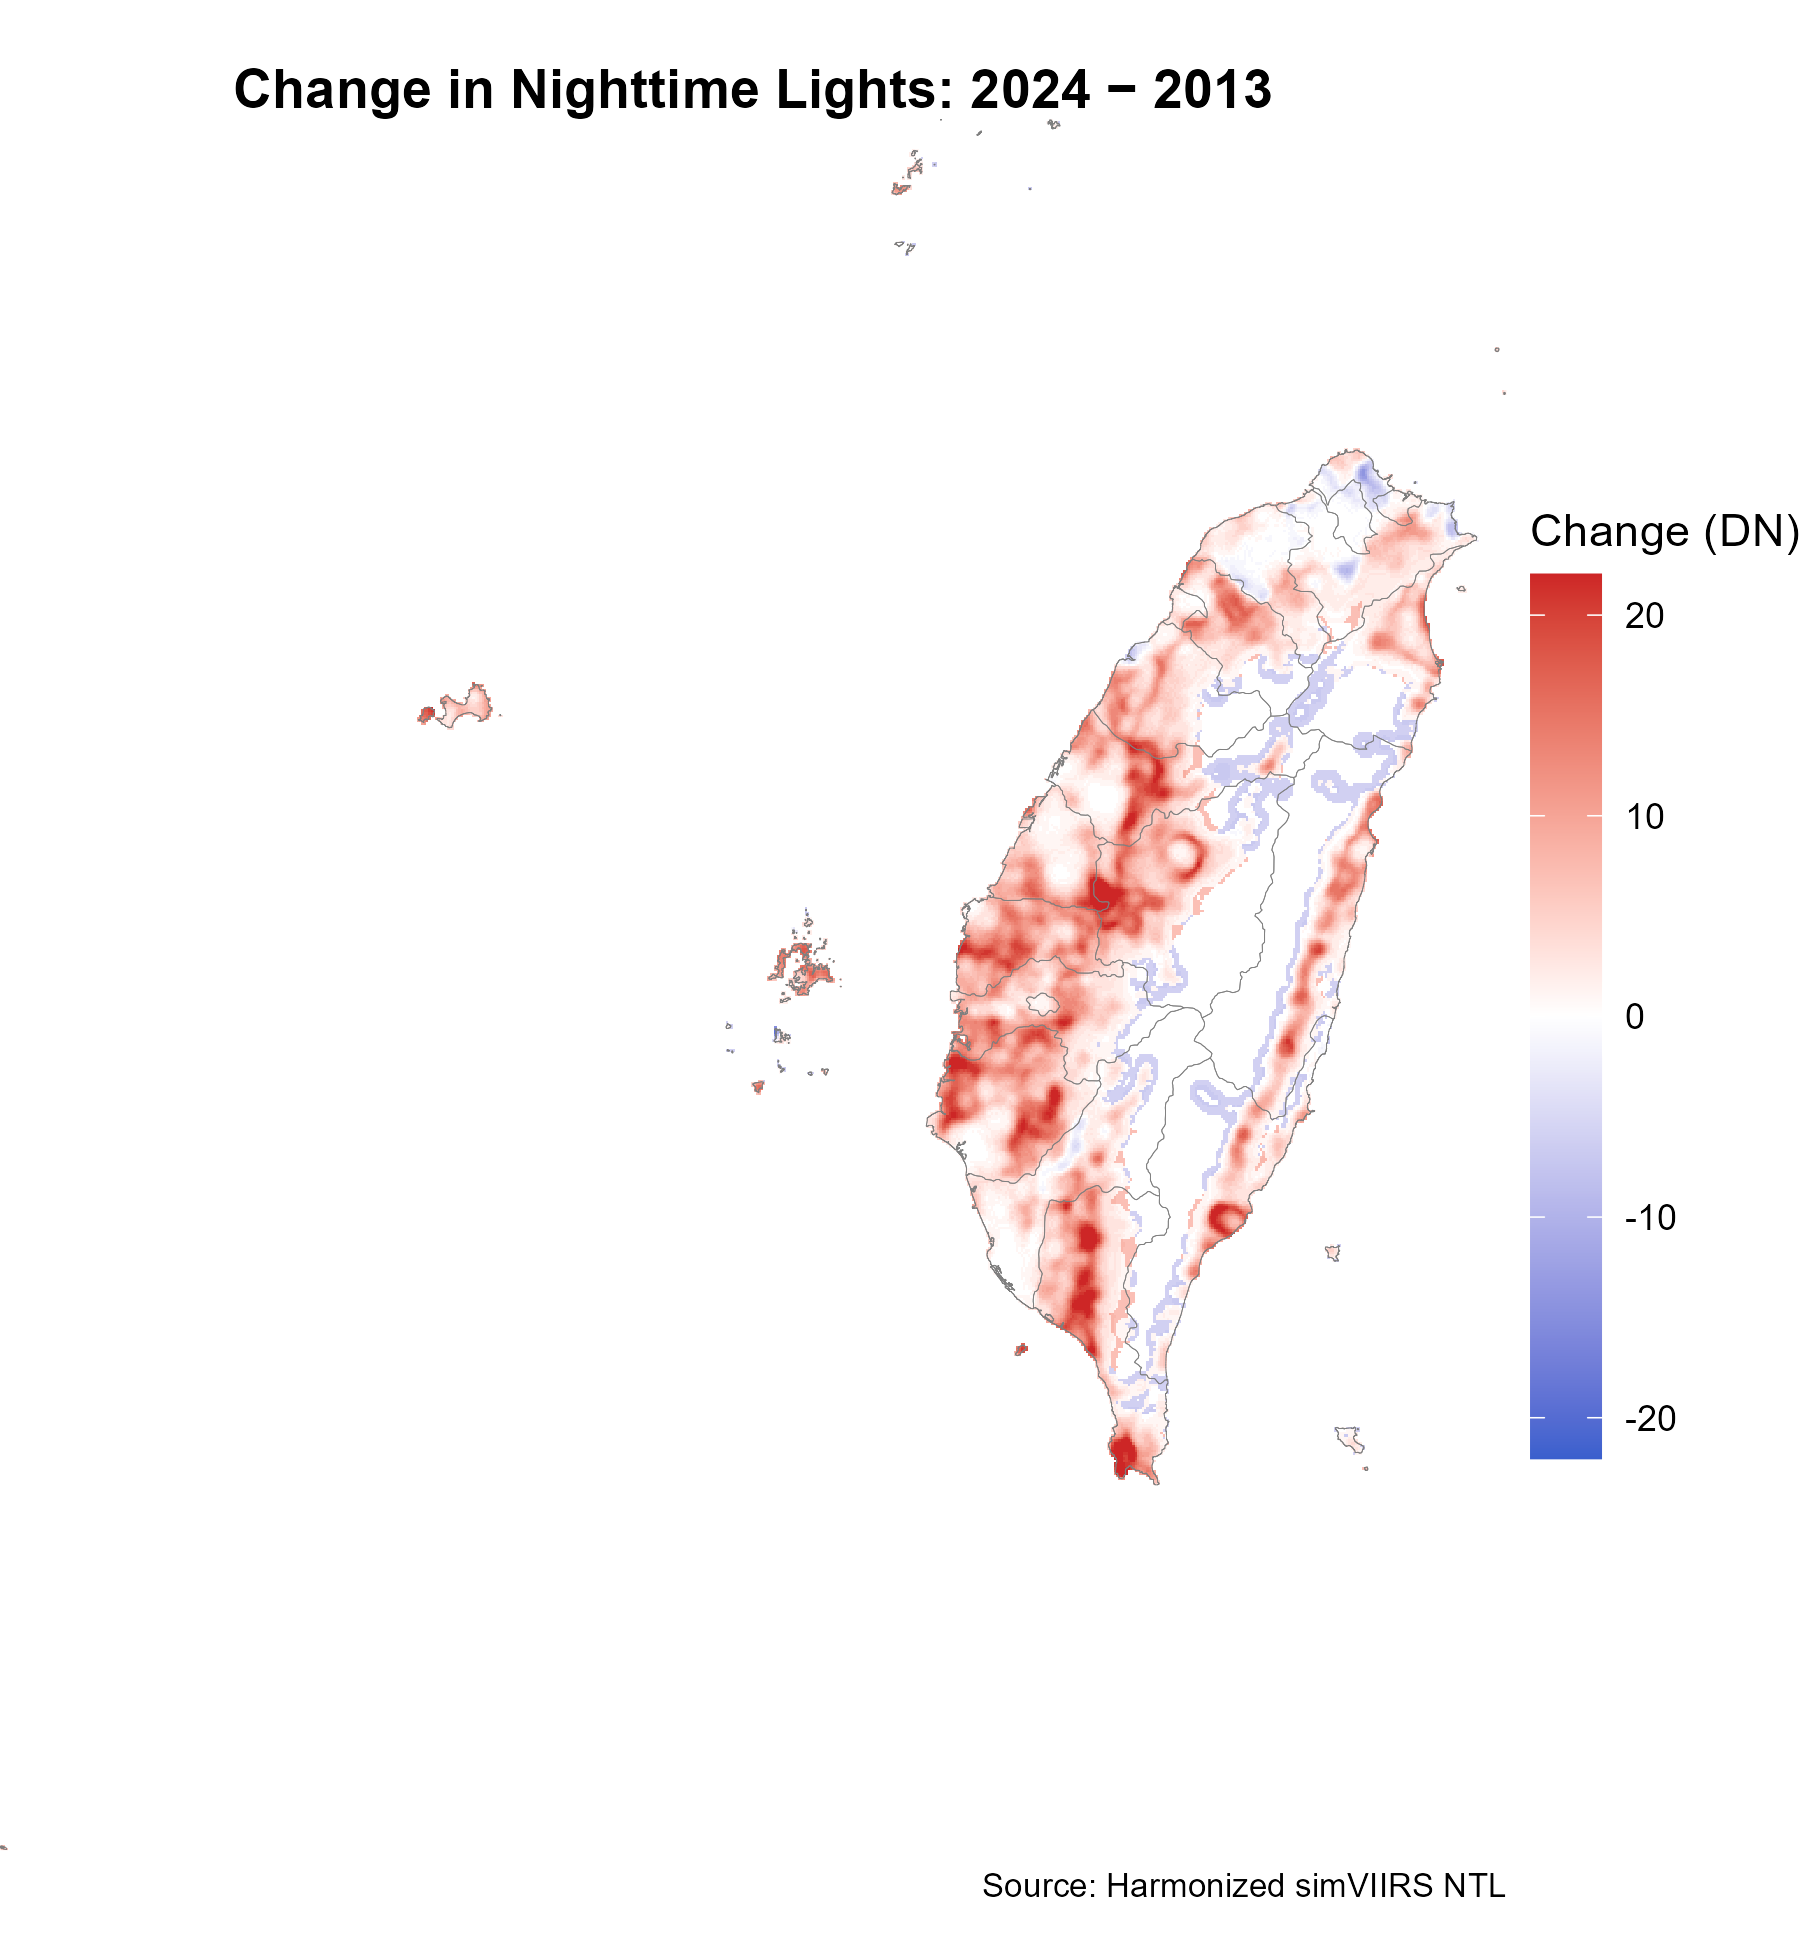
\includegraphics[width=0.78\textwidth]{figure/ntl_taiwan_change_2013_2024.png}
  \end{center}
\end{frame}


\begin{frame}{Township-Level Mean Nighttime Lights}
  \begin{center}
    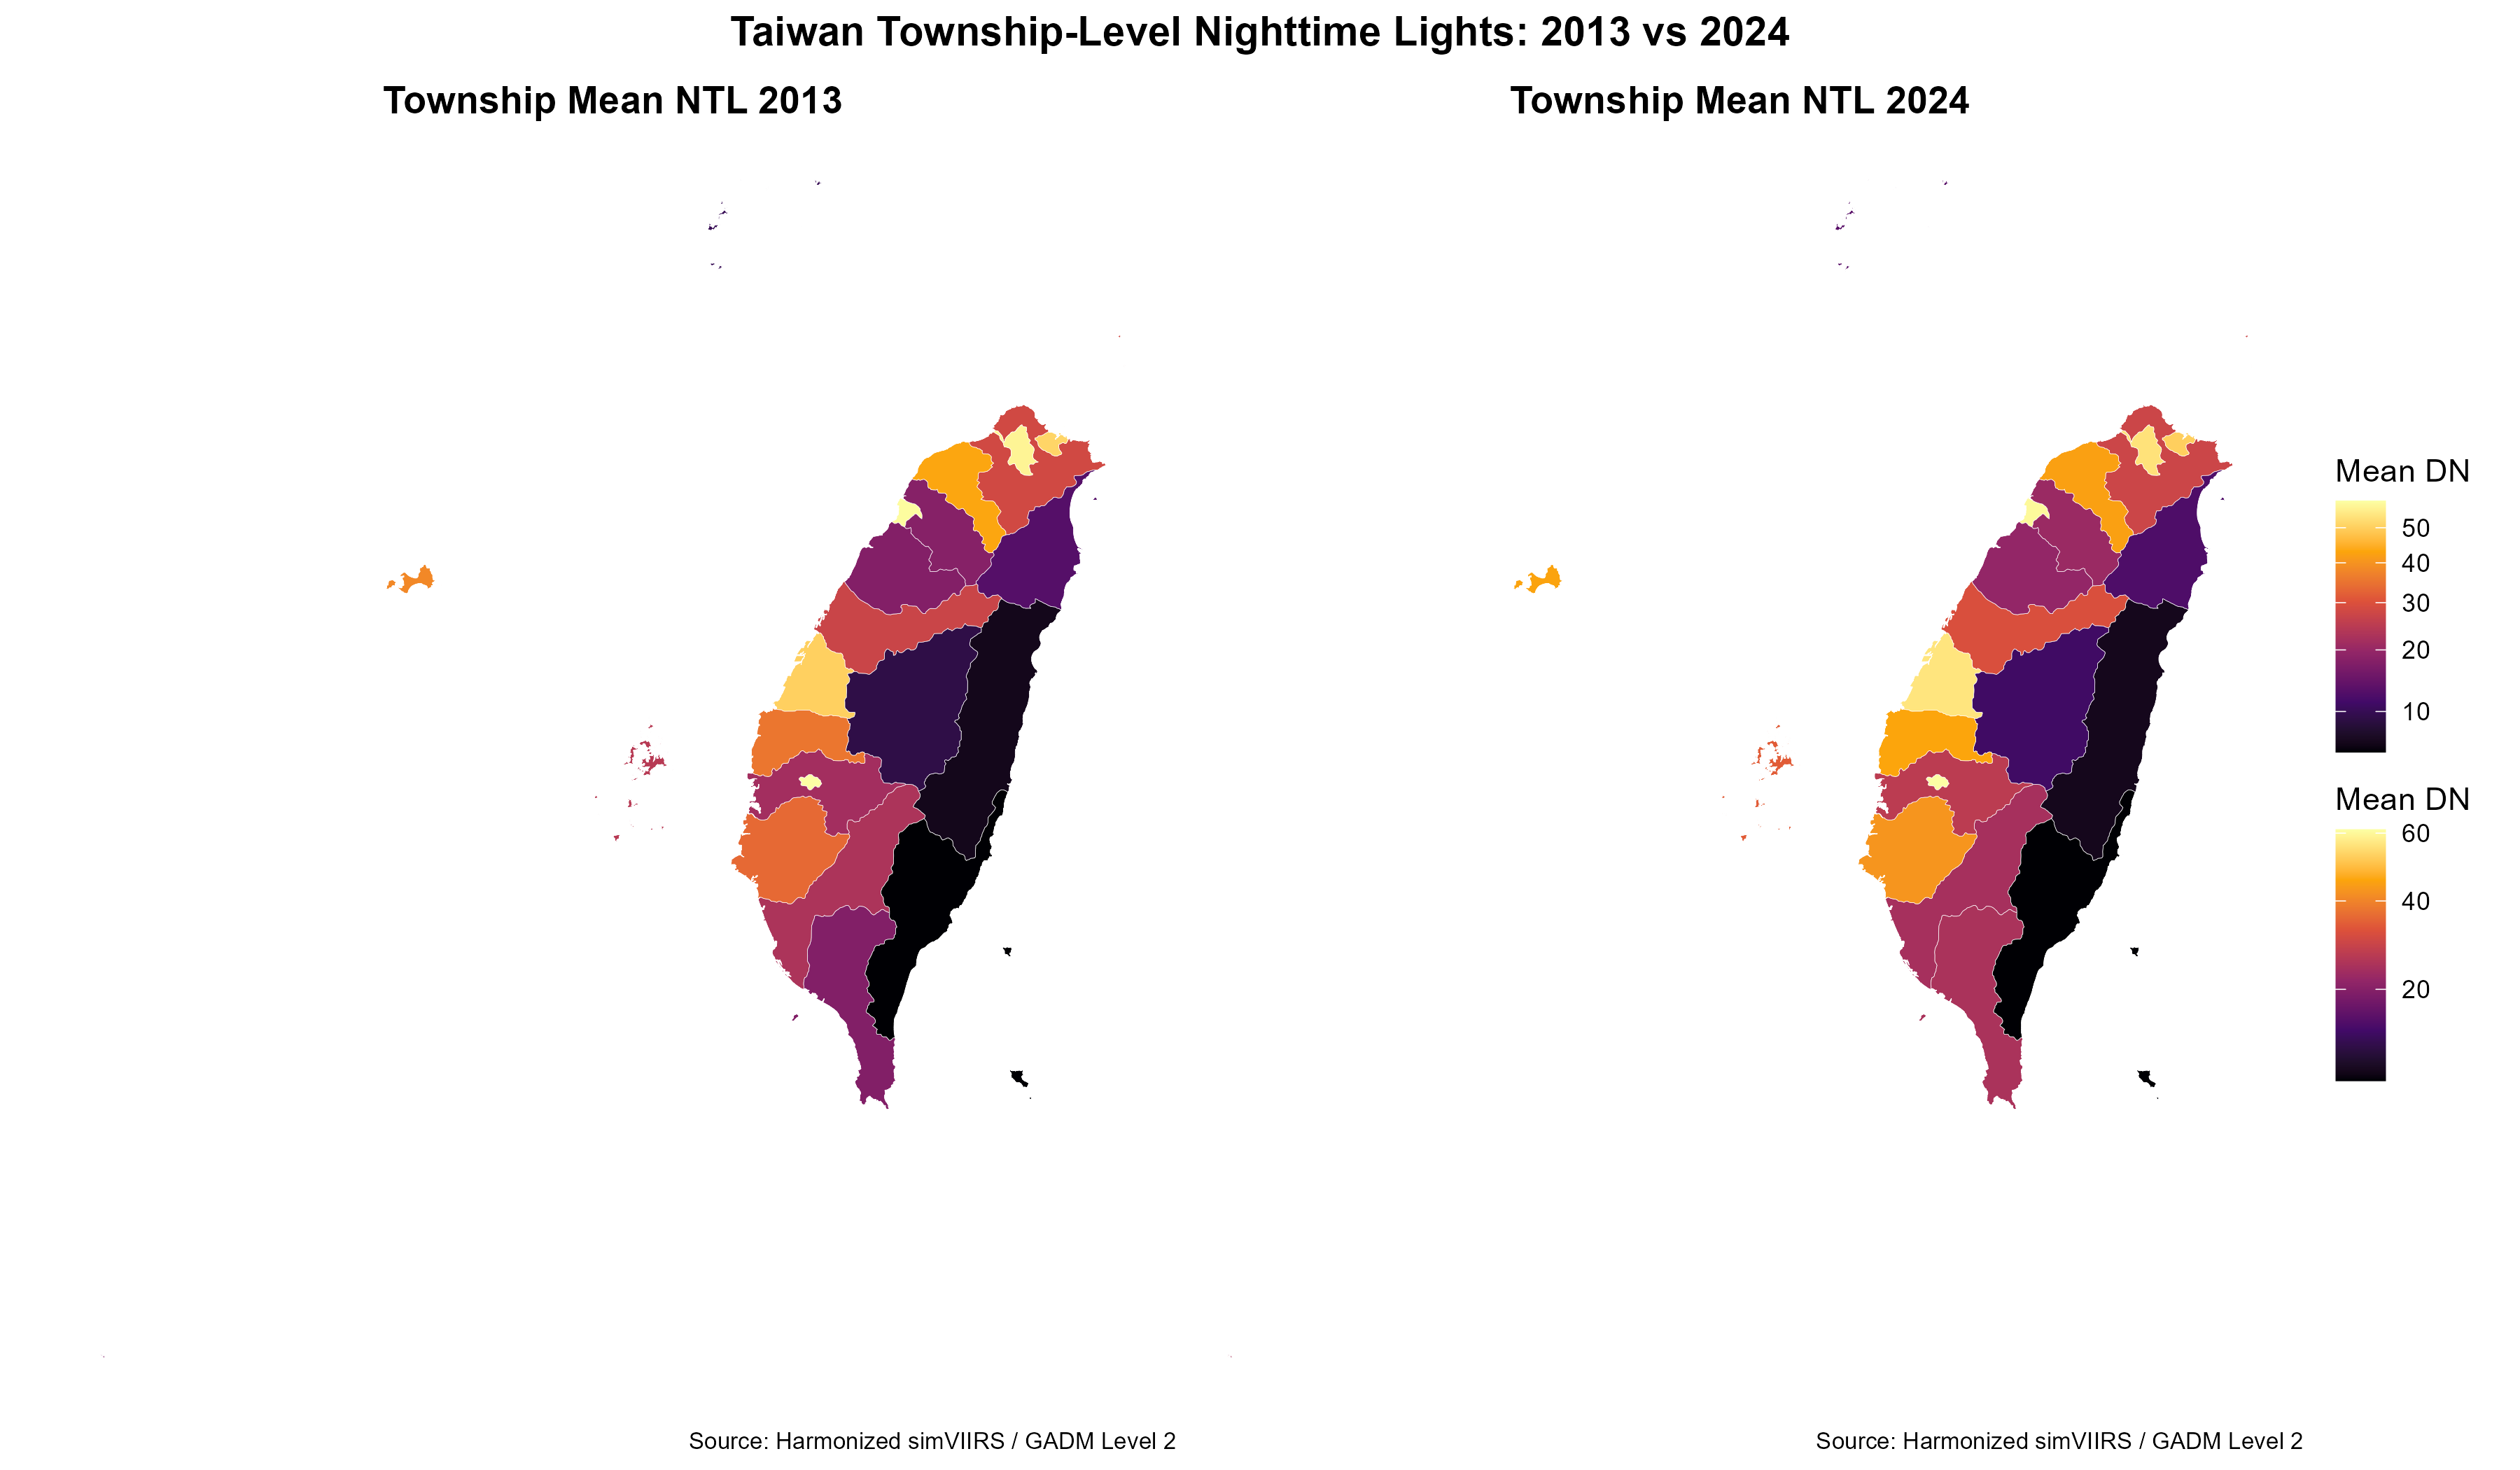
\includegraphics[width=\textwidth]{figure/ntl_township_compare.png}
  \end{center}
\end{frame}


\begin{frame}{Change in Township NTL: 2024 $-$ 2013}
  \begin{center}
    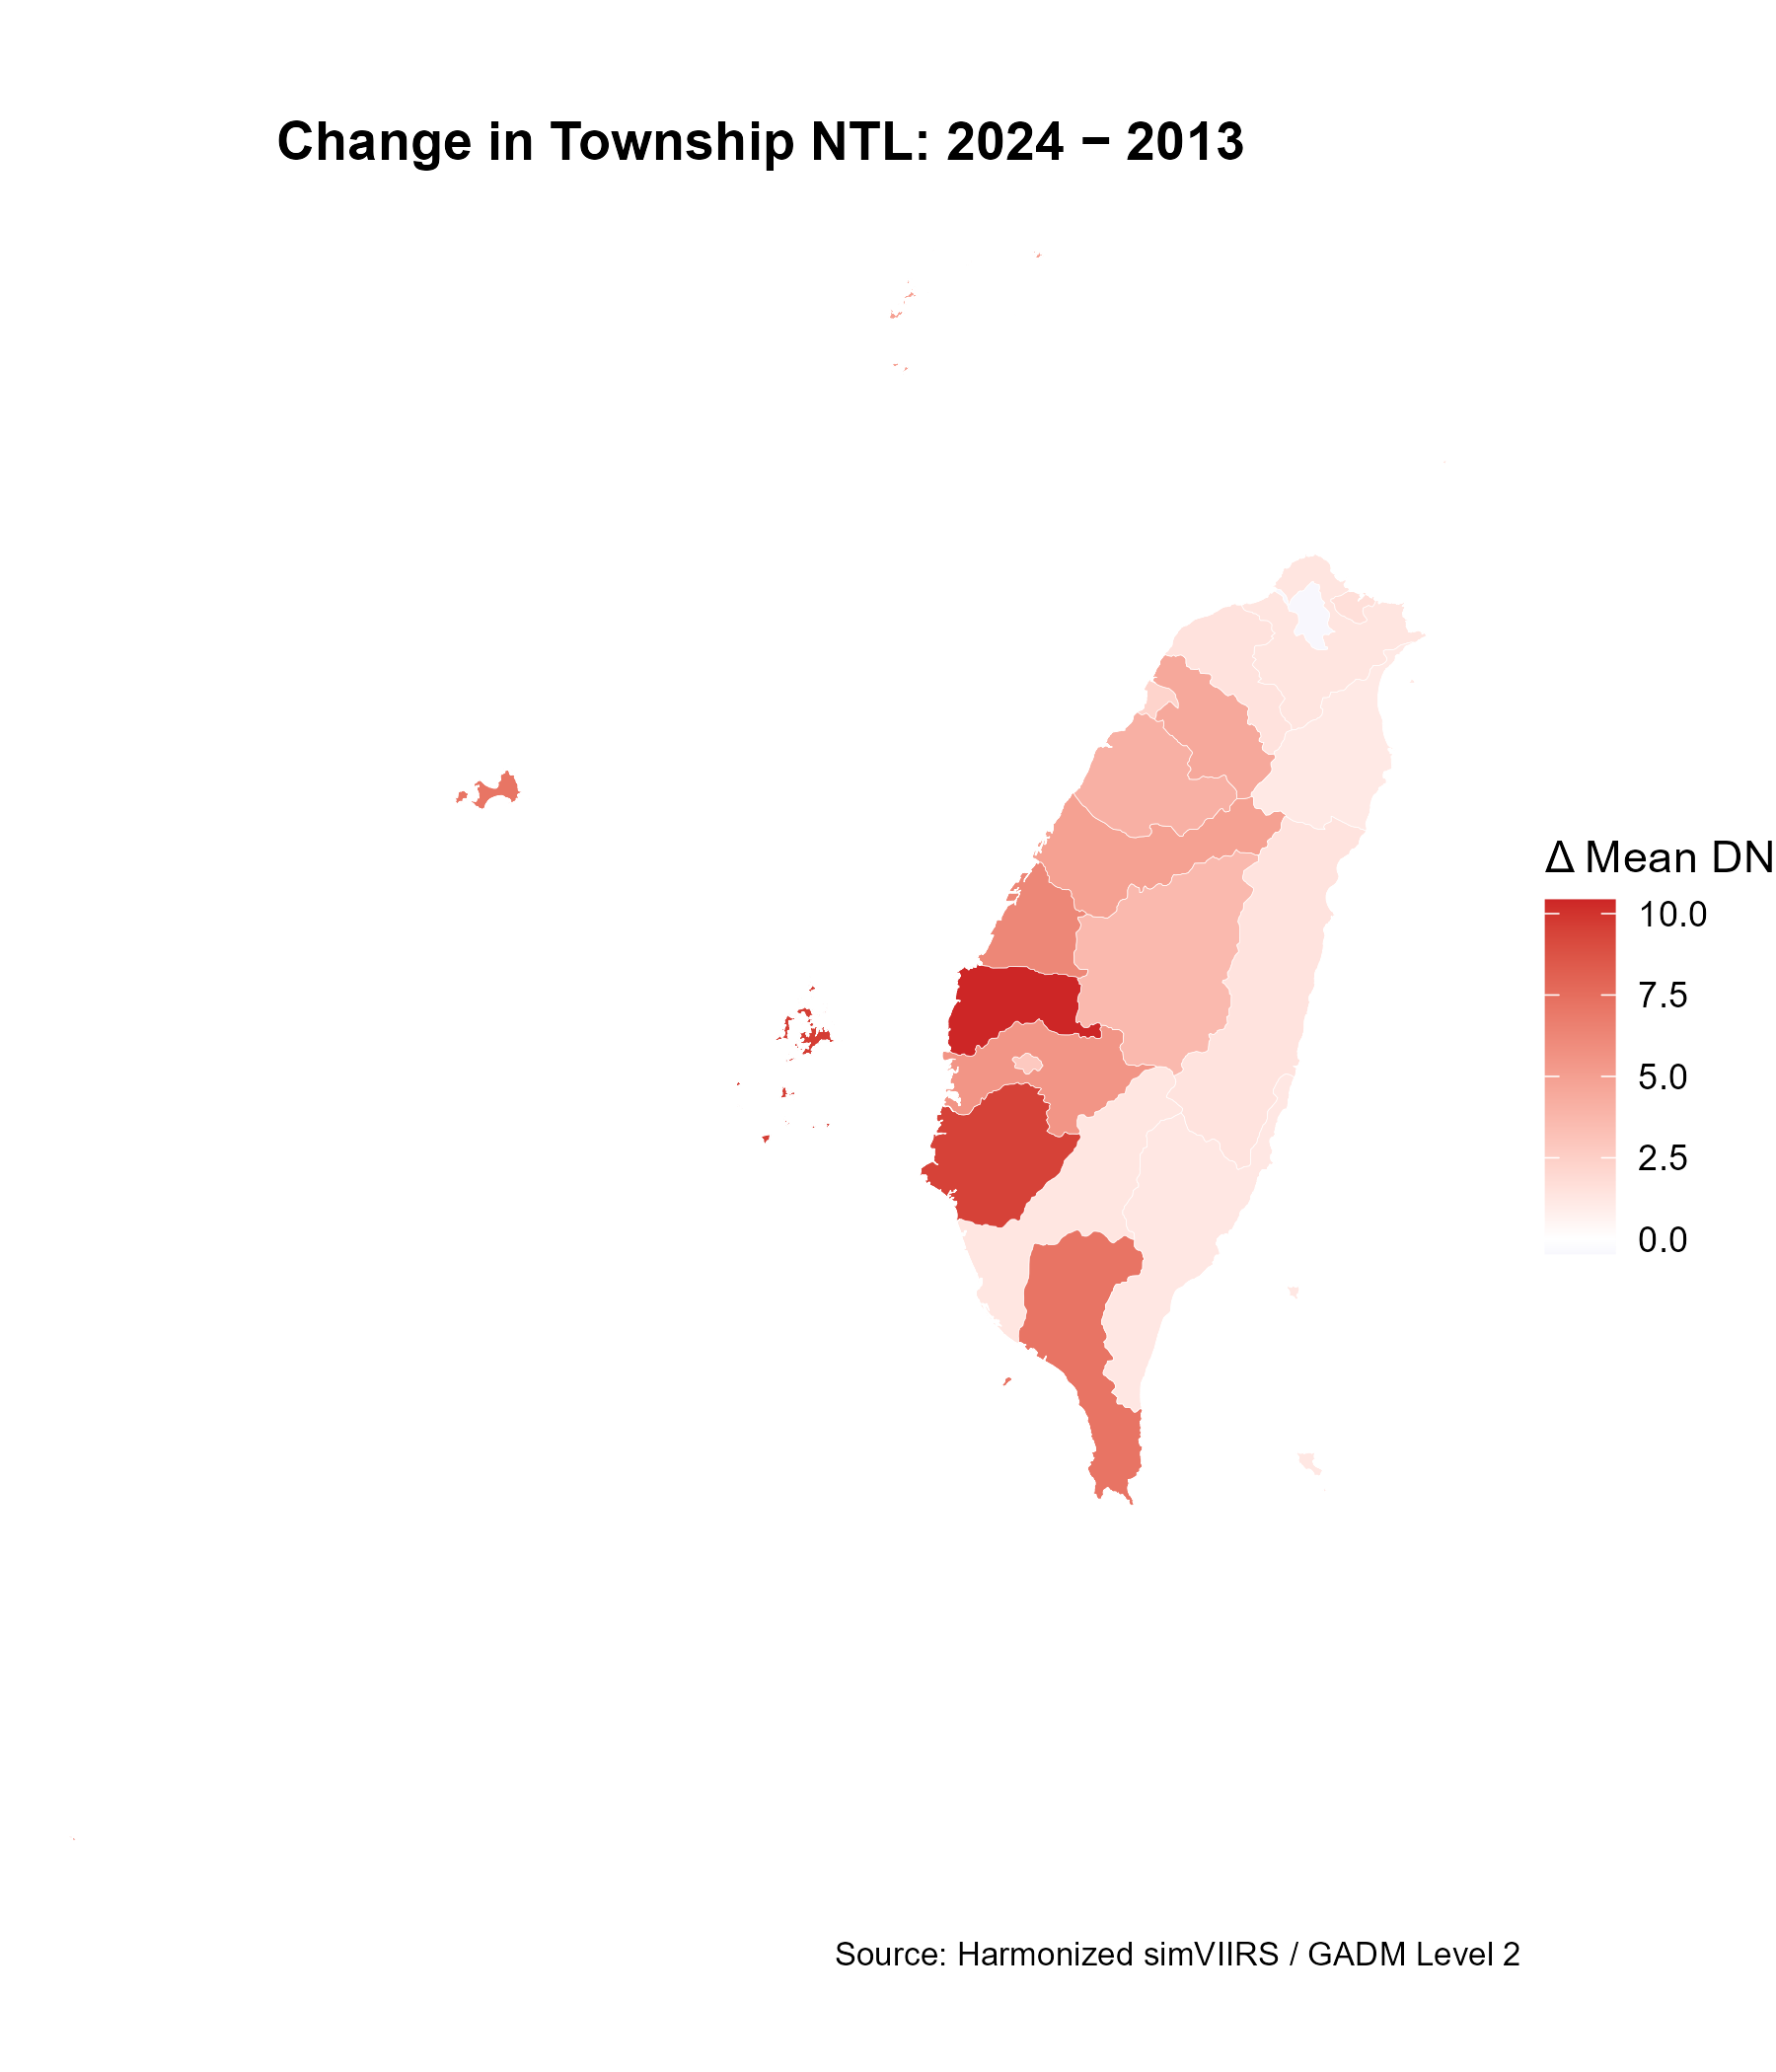
\includegraphics[width=0.72\textwidth]{figure/ntl_township_change.png}
  \end{center}
\end{frame}


\begin{frame}{Township-Level Dataset}
\begin{itemize}
  \item After aggregation, each row is a \textbf{township} (鄉鎮市區),
        $\approx$368 units
  \vspace{0.3cm}
  \item Variables produced (wide format):
  \vspace{0.1cm}
  \begin{center}
  \small
  \begin{tabular}{ll}
    \toprule
    \textbf{Variable}    & \textbf{Description} \\
    \midrule
    \texttt{county}           & County / municipality name \\
    \texttt{township}         & Township / district name \\
    \texttt{ntl\_mean\_2013}  & Mean brightness 2013 (DN) \\
    \texttt{ntl\_sum\_2013}   & Total brightness 2013 \\
    \texttt{ntl\_mean\_2024}  & Mean brightness 2024 \\
    \texttt{ntl\_change\_mean}& Change in mean DN (2024$-$2013) \\
    \texttt{ntl\_pct\_change} & \% change in mean DN \\
    \bottomrule
  \end{tabular}
  \end{center}
  \vspace{0.3cm}
  \item Merge with other township-level variables for regression analysis
\end{itemize}
\end{frame}


%=====================================================================
\title[]{Other Satellite Data}
\author{}
\institute{}
\date{}
\begin{frame}{}
  \titlepage
\end{frame}


\begin{frame}{NDVI: Vegetation Index}
\begin{itemize}
  \item \textbf{What it measures:} the ``greenness'' of land surface ---
        vegetation health and density
  \vspace{0.2cm}
  \[
    \text{NDVI} = \frac{\text{NIR} - \text{Red}}{\text{NIR} + \text{Red}}
    \quad \in [-1,\,+1]
  \]
  \item Higher values $\Rightarrow$ denser, healthier vegetation;
        negative values $\Rightarrow$ water bodies
  \vspace{0.3cm}
  \item \textbf{Data:} NASA MODIS MOD13 (250 m -- 1 km, 16-day or monthly)
  \vspace{0.2cm}
  \item \textbf{R package:} \texttt{MODIStsp} or \texttt{appeears} API
  \vspace{0.3cm}
  \item \textbf{Applications in economics:}
  \vspace{0.1cm}
  \begin{itemize}
    \item Proxy for agricultural productivity and crop yields
    \item Instrument for income shocks in conflict / migration research
  \end{itemize}
\end{itemize}
\end{frame}


\begin{frame}{Land Surface Temperature (LST)}
\begin{itemize}
  \item \textbf{What it measures:} temperature of the Earth's surface
        itself (not air temperature)
  \vspace{0.3cm}
  \item \textbf{Data:} NASA MODIS MOD11A2 (1 km, 8-day composites)
  \vspace{0.2cm}
  \item \textbf{R packages:} \texttt{MODIStsp}, \texttt{appeears}
  \vspace{0.3cm}
  \item \textbf{Applications in economics:}
  \vspace{0.1cm}
  \begin{itemize}
    \item Urban heat islands: link green space and land use to housing prices
    \vspace{0.1cm}
    \item Labor productivity: causal effect of heat on wages and output
    \vspace{0.1cm}
    \item Energy demand: high temperatures raise cooling demand
  \end{itemize}
  \vspace{0.3cm}
  \item \textbf{Advantage over weather stations:}
        globally uniform coverage, no interpolation needed
\end{itemize}
\end{frame}


\begin{frame}{Aerosol Optical Depth (AOD) --- Air Pollution}
\begin{itemize}
  \item \textbf{What it measures:} how much sunlight is blocked by suspended
        particles (PM$_{2.5}$, dust, smoke) across the atmospheric column
  \vspace{0.3cm}
  \item AOD $= 0$: clean atmosphere;\quad AOD $= 1$: heavy particulate loading
  \vspace{0.3cm}
  \item \textbf{Data:} NASA MODIS MOD04 (3 km -- 10 km, daily);
        also available from Sentinel-5P (TROPOMI)
  \vspace{0.2cm}
  \item \textbf{R packages:} \texttt{MODIStsp}, \texttt{sen2r}, \texttt{openeo}
  \vspace{0.3cm}
  \item \textbf{Applications in economics:}
  \vspace{0.1cm}
  \begin{itemize}
    \item Pollution effects on health, cognition, and productivity
    \vspace{0.1cm}
    \item Evaluation of environmental regulations
    \vspace{0.1cm}
    \item Caveat: AOD measures full atmospheric column; conversion to
          ground-level PM$_{2.5}$ requires additional calibration
  \end{itemize}
\end{itemize}
\end{frame}


\begin{frame}{Summary: Satellite Data Packages in R}
\begin{center}
\small
\begin{tabular}{lll}
  \toprule
  \textbf{Data} & \textbf{R Package} & \textbf{Source} \\
  \midrule
  Nighttime lights    & \texttt{blackmarbler}    & NASA LAADS DAAC \\
  NDVI / LST / AOD    & \texttt{MODIStsp}        & NASA MODIS \\
                      & \texttt{appeears}         & NASA AppEEARS API \\
  Sentinel-2 imagery  & \texttt{sen2r}            & ESA / Copernicus \\
  Google Earth Engine & \texttt{rgee}             & Google EE \\
  Harmonized NTL      & (direct download)         & Li et al.\ (2020) \\
  Elevation (DEM)     & \texttt{elevatr}          & USGS / Amazon \\
  Population          & \texttt{wpgpDataR}        & WorldPop \\
  \bottomrule
\end{tabular}
\end{center}
\vspace{0.3cm}
\begin{itemize}
  \item All sources are free; most require a one-time account registration
  \item See also: \href{https://earthdata.nasa.gov}{\texttt{earthdata.nasa.gov}}
        and \href{https://browser.dataspace.copernicus.eu}{\texttt{Copernicus Browser}}
\end{itemize}
\end{frame}


\end{document}
